\chapter{Zastosowanie znaczników radiowych do mierzenia odległości}
\label{ch:radio}
Systemy nawigacji satelitarnej takie jak GPS czy GLONASS, jak i systemy lokalizacji za pomocą sieci komórkowej nie znajdują zastosowania w lokalizacji wewnątrz pomieszczeń. Podstawowymi problemami, na jakie natrafiają te systemy, jest brak zasięgu wewnątrz pomieszczeń i związana z tym zbyt mała dokładność.
Jednocześnie popularyzacja sieci Wi-Fi i standardu komunikacji bezprzewodowej Bluetooth spowodowała, że urządzenia wykorzystujące te standardy są szeroko dostępne i przystępne cenowo. Sieci Wi-Fi i standard Bluetooth operują paśmie ISM (Industrial, Scientific and Medical, częstotliwości rzędu 2.4 GHz). Dobra dostępność tych technologii skłania do wykorzystania ich także w robotyce. 

W niniejszym rozdziale przedstawiono podstawy teoretyczne modelu propagacji fal radiowych w pomieszczeniu, następnie opisano problem modelowania relacji odległość - siła sygnału i możliwe jego rozwiązania. Przedstawiono także najpopularniejsze technologie radiowe pasma ISM, z naciskiem na technologię Bluetooth, wybraną do implementacji rozwiązania. 

\section{Propagacja sygnału radiowego w pomieszczeniu zamkniętym}
Do szacowania poziomu sygnału w modelach propagacyjnych wprowadza się parametr zwany współczynnikiem tłumienności trasy. Opisuje on zmniejszenie poziomu sygnału odbieranego w stosunku do mocy sygnału nadawanego w skutek przejścia fal radiowych przez środowisko propagacyjne wprowadzające pewne tłumienie. Transmisję sygnału radiowego opisuje schemat przedstawiony na rys. \ref{fig:propagacja-fal}. Przez $P_{TX}$ oznaczono moc nadajnika, $G_{TX}$ - zysk anteny nadawczej, $G_{RX}$ - zysk anteny odbiorczej, $L$ - współczynnik tłumienności trasy (ang. \textit{path loss index}), zaś $P_{RX}$ - moc sygnału odebranego \cite{rssi}. 

Współczynnik $L$ opisuje własności propagacyjne środowiska, w którym przekazywany jest sygnał. Obejmuje zatem czynniki takie jak tłumienność trasy, obecność ścian budynków lub innych przeszkód terenowych, obecność innych źródeł promieniowania. Związane z wymienionymi czynnikami zjawiska odbicia, dyfrakcji i interferencji sygnału powodują, że zagadnienie wyznaczenia współczynnika tłumienności jest niezwykle trudne. W związku z tą trudnością, najczęściej stosowane są modele empiryczne, a zatem oparte na pomiarach siły sygnału w danym środowisku. 

Relację mocy sygnału nadanego i mocy odebranej przez odbiornik można wyrazić następująco: 
\begin{equation}
\label{eq:L}
 L = P_{TX} - P_{RX}
\end{equation}

Do obliczenia odległości na podstawie siły sygnału RSSI (ang. \textit{Received Signal Strength Indicator}, wskaźnik siły sygnału sygnału odebranego) należy posłużyć się modelem propagacji:
\begin{equation}
\label{eq:model_propag}
 P_{RX} = P_{TX}+G_{TX}+G_{RX} + 20\log(\lambda) - 20\log(4\pi) -10n\log(d)
\end{equation}

W równaniu \ref{eq:model_propag} przez $d$ oznaczono odległość między transmiterem a odbiornikiem, $\lambda$ oznacza długość fali, zaś współczynnik $n$ określa wpływ przeszkód takich jak ściany. Należy zaznaczyć, że wartości mocy nadajnika $P_{TX}$, zysków anten $G_{RX}$ i $G_{TX}$, długości fali $\lambda$ oraz współczynnika $n$ na ogół nie są znane, podczas gdy moc sygnału odebranego $P_{RX}$ jest zwykle możliwa do określenia, jako że implementacje protokołów radiowych przewidują dołączenie jej wartości do zdekodowanych ramek danych. 

Ponadto, wyznaczenie analityczne współczynnika $n$ jest niemożliwe. Zależy on bowiem bardzo silnie od architektury pomieszczenia, położenia nadajnika względem ścian, podłogi i stropu, a także od zakłóceń. Jako podstawowe źródła zakłóceń sygnału można wyróżnić:

\begin{itemize}
 \item odbiorniki elektryczne dużej mocy, np. kuchenki lub silniki elektryczne,
 \item silne źródła promieniowania, takie jak kuchenki mikrofalowe,
 \item inne nadajniki radiowe korzystające z danego pasma, szczególnie bardzo popularne punkty dostępowe sieci Wi-Fi.
\end{itemize}

Obecność ścian, przedmiotów a także obiektów ruchomych, np. przemieszczających się ludzi, powoduje występowanie odbić i rozproszeń fali radiowej. Pod pewnymi względami może zajść także tzw. efekt falowodowy, wskutek którego fala pokonuje znacznie większą odległość bez tłumienia (dzieje się tak np. w długich korytarzach). Powyższe zjawiska skutkują wzrostem zjawiska wielokrotnego obicia, czyli docierania fali do odbiornika wieloma drogami (np. bezpośrednio z nadajnika i po odbiciu od ściany). To zjawisko jest szczególnie poważną przeszkodą do zastosowania pomiaru siły sygnału RSSI do wyznaczenia odległości. 

\begin{figure}[H]
\centering
\includegraphics[width=0.7\textwidth]{img/propagacja-fal.png}
\caption{Schemat propagacji fal radiowych}
\label{fig:propagacja-fal}
\end{figure}

\section{Wyznaczanie odległości na podstawie siły sygnału RSSI}
\label{sec:rssi-odleglosc}
Zgodnie z zależnością \ref{eq:model_propag}, wraz ze wzrostem odległości nadajnika i odbiornika, wartość RSSI powinna spadać. Jednakże z powodu zjawisk wymienionych w poprzedniej sekcji, ta zależność nie zawsze jest zachowana. Dla odbiornika pozostającego w stałej odległości od nadajnika, wartość RSSI nie pozostaje stała, co obrazują wyniki eksperymentalne (wykres na rys. \ref{fig:rssi-stacjonarne}). 

\begin{figure}[H]
\centering
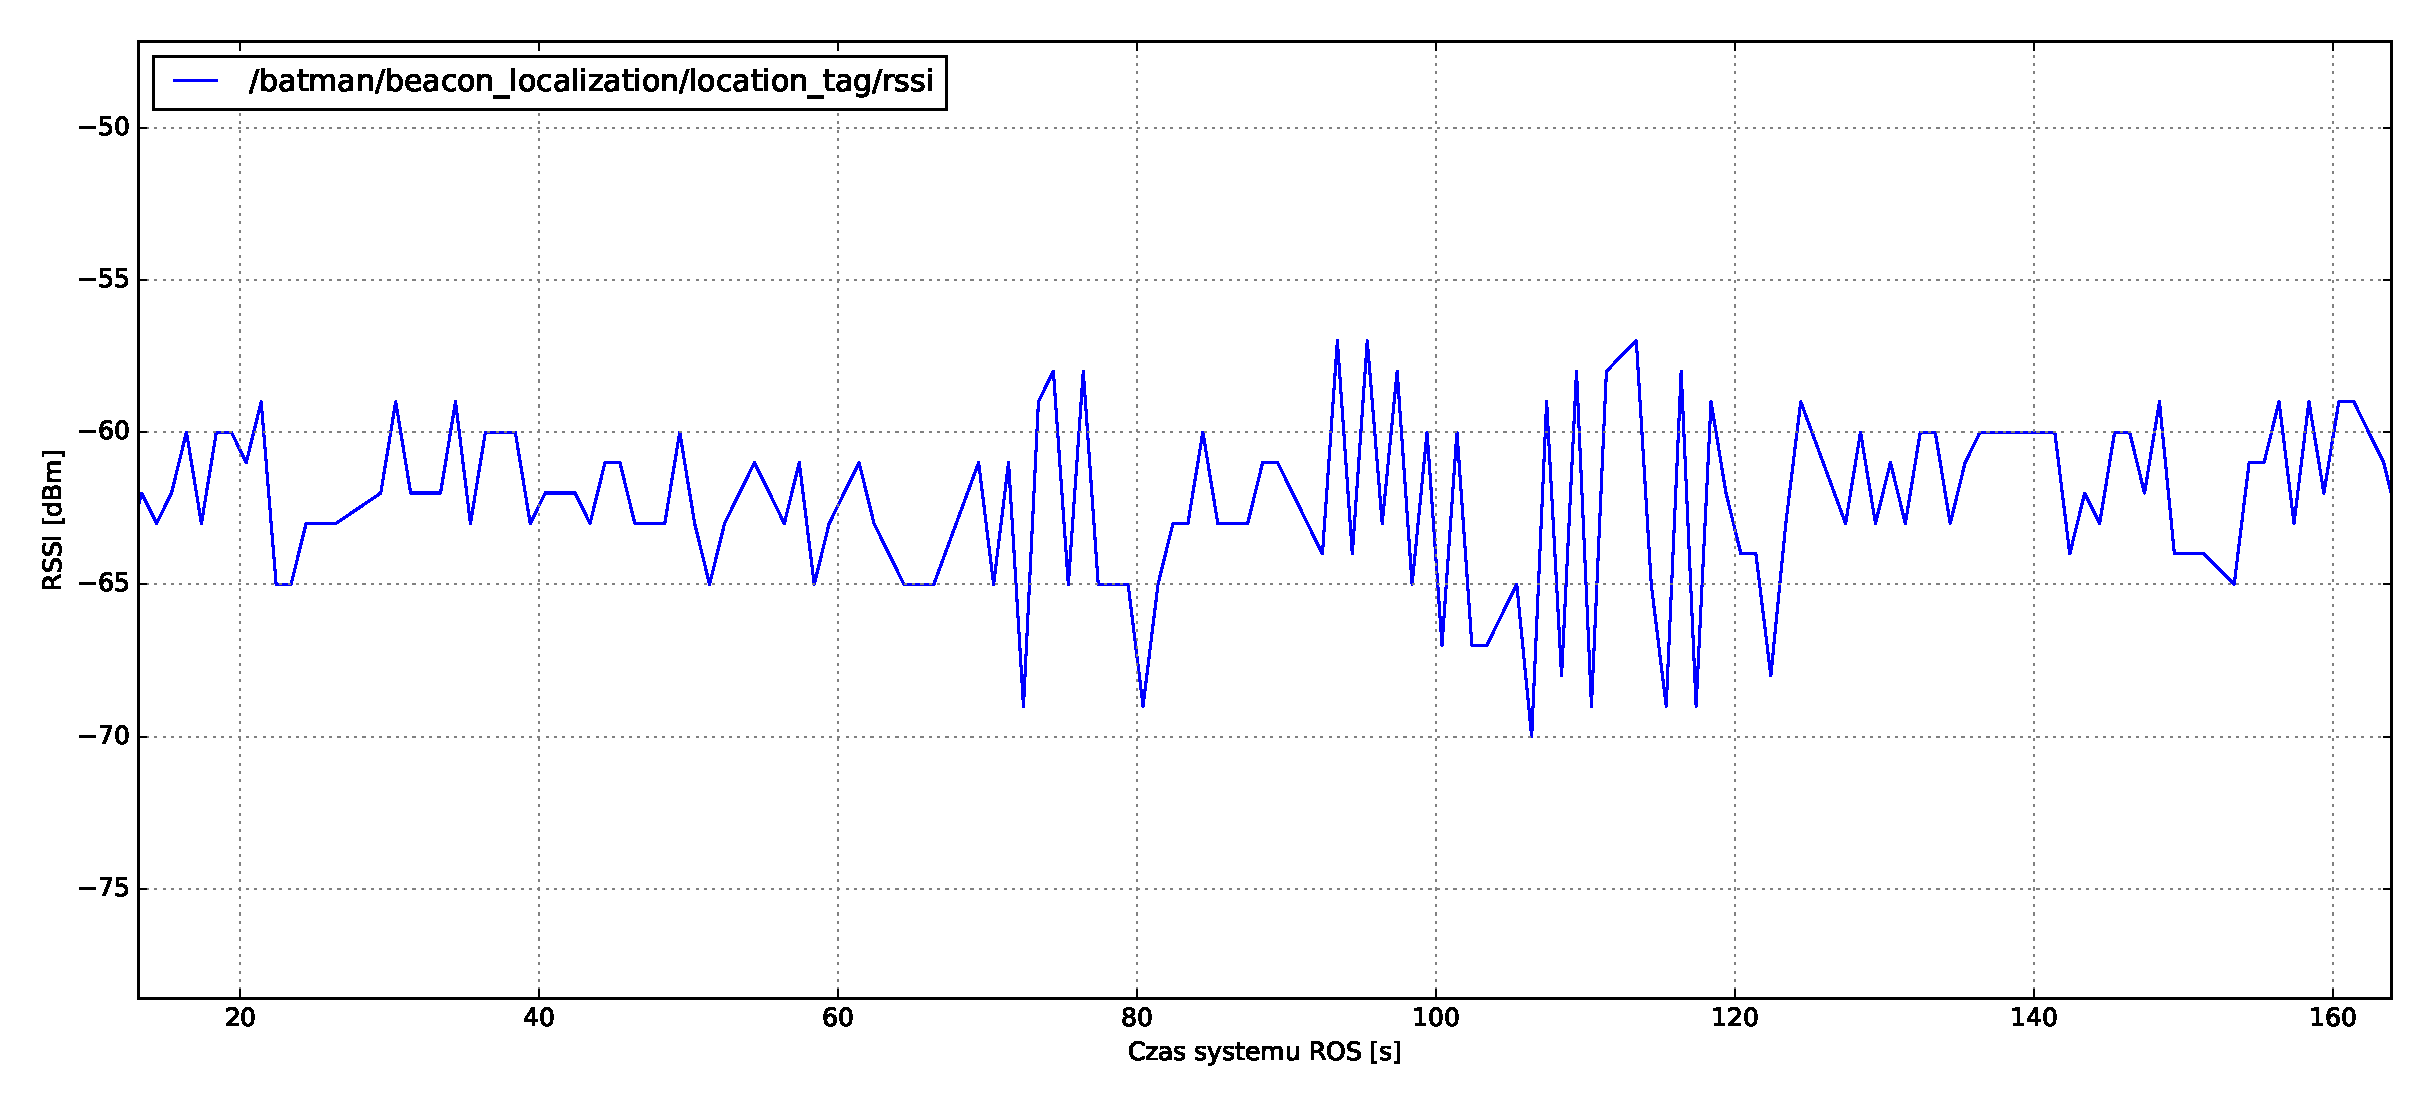
\includegraphics[width=0.85\textwidth]{img/rssi_stacjonarne.eps}
\caption{Przebieg wartości RSSI dla stacjonarnego odbiornika będącego w odległości 70 cm od nadajnika (znacznik BLE). Pominięto pierwsze 15 sekund pomiaru ze względu na stan nieustalony systemu ROS.}
\label{fig:rssi-stacjonarne}
\end{figure}

Jak widać z wykresu \ref{fig:rssi-stacjonarne}, nawet dla nieruchomego odbiornika występują wahania RSSI rzędu 10 dBm. Dlatego konieczne jest zastosowanie filtra wygładzającego. Do wygładzenia wartości RSSI można wykorzystać następujące narzędzia:
\begin{itemize}
 \item filtr oparty o średnią ruchomą prostą lub ważoną,
 \item filtr dolnoprzepustowy,
 \item filtr Kalmana, uwzględniający wiedzę na temat ruchu odbiornika.
\end{itemize}

Projektując filtr RSSI, należy zwrócić szczególną uwagę na bezwładność, jaką wprowadza on do pomiaru, a która utrudnia lub nawet uniemożliwia pomiar odległości dla odbiornika pozostającego w ruchu. W tym kontekście, szczególnie użyteczny jest filtr Kalmana, który może wykorzystać informację o ruchu odbiornika radiowego pochodzącą np. z systemu lokalizacji robota. Szczegóły dotyczące filtracji sygnału RSSI zostały szerzej omówione w rozdziale \ref{ch:metody-lokalizacji}, gdzie opisano proponowany algorytm lokalizacji robota.

Kolejnym problemem związanym z pomiarem odległości za pomocą siły sygnału RSSI jest wyznaczenie zależności siły sygnału RSSI od odległości $P_{RX}(d)$. Wzór \ref{eq:model_propag} zawiera parametry nadajnika i odbiornika oraz medium transmisyjnego, które na ogół nie są znane. Z pomocą przychodzą metody empiryczne. Wykonując serię pomiarów siły sygnału w różnych odległościach od nadajnika i w różnych miejscach pomieszczenia, otrzymuje się zbiór danych który pozwala na wyznaczenie aproksymacji zależności $P_{RX}(d)$. W dalszej części rozdziału opisano podstawowe metody otrzymywania tej aproksymacji.

\subsection{Aproksymacja za pomocą krzywych wielomianowych}
Pierwszym możliwym rozwiązaniem jest dopasowanie krzywej wielomianowej do punktów pomiarowych, proponowane przez autorów artykułu \cite{rssi}. Aproksymowana funkcja ma postać:
\begin{equation}
\label{eq:approx_poly}
  y_{P_{RX}} = a_0 + a_1 d_x + a_2 d_x^2 + ... + a_n d_x^n
\end{equation}

gdzie $a_0, ..., a_n$ są współczynnikami wielomianu stopnia $n$, aproksymującego zależność. Mając $N$ punktów pomiarowych $(d_{xi}, y{P_{RX}i})$, gdzie $i = 1,2, ..., N$, błąd aproksymacji $e_i$ wynosi

\begin{equation}
\label{eq:approx_poly_e}
  e_i = y_{P_{RX}} -( a_0 + a_1 d_x + a_2 d_x^2 + ... + a_n d_x^n )
\end{equation}

Współczynniki $a_0, ..., a_n$ wyznacza się rozwiązując zadanie minimalizacji błędu średniokwadratowego:

\begin{equation}
\label{eq:approx_poly_mse}
  S = \sum_{i=1}^{N} e_i^2
\end{equation}

Wyniki przedstawione w artykule \cite{rssi} wskazują, że najlepsze wyniki dają aproksymacje wielomianami niskiego rzędu $n=2, n=3$

\subsection{Interpolacja}
Kolejną metodą aproksymowania zależności $P_{RX}(d)$ proponowaną przez \cite{rssi} jest interpolacja. Pozwala ona na wyeliminowanie niewiadomych składników równania. Rozważmy dwa wybrane pomiary. Oznaczając je indeksami 1 i 2 oraz podstawiając do równania \ref{eq:model_propag} otrzymujemy:

\begin{equation}
\label{eq:interpol_podst1}
 P_{RX1} = P_{TX}+G_{TX}+G_{RX} + 20\log(\lambda) - 20\log(4\pi) -10n\log(d_1)
\end{equation}
\begin{equation}
\label{eq:interpol_podst2}
 P_{RX2} = P_{TX}+G_{TX}+G_{RX} + 20\log(\lambda) - 20\log(4\pi) -10n\log(d_2),
\end{equation}
gdzie $P_{RX}$ jest mocą odebranego sygnału, $P_{TX}$ - mocą sygnału nadawanego, $G_{RX}$ i $G_{TX}$ odpowiednio wzmocnieniem anteny odbiorczej i nadawczej, $\lambda$ - długością fali sygnału radiowego, zaś $d$ - odległością odbiornika od nadajnika. 

Odjęcie powyższych równań stronami pozwala wyeliminować niewiadome zależne od sprzętowych aspektów nadajnika i odbiornika, a następnie wyprowadzić zależność interpolowaną postaci:
\begin{equation}
\label{eq:interpol}
 P_{RX} = (P_{RX1}-P_{RX2}) \frac{\log{d} - \log{d_2}}{\log{d_1} - \log{d_2}} + P_{RX2}
\end{equation}

Wykorzystując dwa punkty pomiarowe i zależność \ref{eq:interpol} można otrzymać aproksymację zależności RSSI od odległości. Punkty do interpolacji należy dobrać eksperymentalnie, aby osiągnąć optymalne wyniki. 

\subsection{Dopasowanie krzywej logarytmicznej lub wykładniczej}
Łatwo zauważyć, że w równaniu \ref{eq:model_propag} część składników jest stała i zależy od uwarunkowań sprzętowych nadajnika i odbiornika, bądź warunków środowiskowych. Grupując składniki stałe można napisać:

\begin{equation}
\label{eq:logfit}
 P_{RX} = A + B \log(d)
\end{equation}

gdzie:

\begin{equation}
\label{eq:logfitA}
A = P_{TX}+G_{TX}+G_{RX} + 20\log(\lambda) - 20\log(4\pi)
\end{equation}

\begin{equation}
\label{eq:logfitB}
B = -10n
\end{equation}

Wykorzystując narzędzia optymalizacyjne, dostarczane przez pakiety takie jak MATLAB lub bibliotekę SciPy można wykonać dopasowanie krzywej logarytmicznej do punktów pomiarowych, aby otrzymać zależność postaci \ref{eq:logfit} \cite{scipy}. Dokonując odpowiednich przekształceń, można łatwo wyznaczyć także zależność odwrotną, faktycznie potrzebną w zadaniu lokalizacji. Ma ona postać:

\begin{equation}
\label{eq:logfit_d}
d = 10 ^ {\frac{P_{RX}-A}{B}}
\end{equation}

W dalszej części rozdziału opisano popularne technologie radiowe, możliwe do wykorzystania w lokalizacji robota mobilnego. 

\section{Protokół Wi-Fi}
\label{sec:wifi}
Nazwa Wi-Fi (ang. Wireless Fidelity, \textit{Bezprzewodowa wierność}) jest potocznym określeniem zestawu standardów określających budowę bezprzewodowych sieci komputerowych, w szczególności sieci WLAN, czyli bezprzewodowych sieci lokalnych. Wi-Fi wykorzystuje częstotliwości pasma ISM: 2.4 GHz oraz 5.8 GHz. Warstwa fizyczna oraz podwarstwa MAC jest opisywana przez grupę standardów IEEE 802.11. Duża popularność sieci Wi-Fi w budynkach sprawia, że rozwiązanie to dobrze nadaje się do zastosowania w lokalizacji. Istnieje szereg opracowań naukowych wykorzystujących technologię Wi-Fi do lokalizacji wewnątrz pomieszczeń (\cite{fingerprinting}), nie tylko w robotyce, ale także m. in. do lokalizowania osób posiadających telefon komórkowy (\cite{rssi}). Zasilanie sieciowe punktów dostępych pozwala na szybkość transmisji danych znacznie większą niż w innych technologiach radiowych. Jednakże, wadą rozwiązania jest duże zużycie energii, szczególnie po stronie odbiornika który często zasilany jest bateryjnie, oraz koszt urządzeń i ich instalacji większy niż w wypadku opisanego dalej Bluetooth. 


\section{Protokół Bluetooth}
\label{sec:bluetooth}
Bluetooth jest standardem komunikacji bezprzewodowej, zaprojektowanym do wymiany danych na krótkie dystanse, korzystający z fal krótkich UHF pasma ISM (częstotliwości rzędu 2.4 GHz). Standard Bluetooth jest zarządzany przez organizację Bluetooth Special Interest Group (SIG), będącą zrzeszeniem firm z branż komunikacyjnej, sieciowej, informatycznej i elektronicznej \cite{ble}. 

Pasmo ISM (ang. \emph{Industrial, Scientific and Medical}, Przemysłowe, Naukowe i Medyczne) wykorzystywane przez Bluetooth jest nielicencjonowane. Dla zapewnienia odporności na zakłócenia, Bluetooth wykorzystuje technologię rozpraszania widma FHSS (ang. \emph{Frequency Hopping Spread Spectrum}) polegającą na "skakaniu" po częstotliwościach dostępnych w paśmie w kolejnych odstępach czasu. Protokół Bluetooth jest oparty o pakiety, ze strukturą master-slave \cite{ble}. 

\subsection{Bluetooth Low Energy}
\label{sec:ble}
Bluetooth Low Energy, znane także pod nazwą handlową Bluetooth Smart, jest czwartą wersją specyfikacji standardu Bluetooth. Standard ten został zorientowany na zapewnienie transmisji o minimalnym koszcie energetycznym. Podstawowe cechy BLE to: 
\begin{itemize}
 \item niskie zużycie energii, pozwalające urządzeniom operować przez długi (rzędu roku) czas na jednej baterii guzikowej,
 \item mały rozmiar i koszt urządzeń,
 \item kompatybilność z popularnymi urządzeniami obecnymi na rynku (smartfony, tablety, laptopy).
\end{itemize}

Dla osiągnięcia efektywności energetycznej BLE wykorzystuje odmienny w stosunku do klasycznego Bluetooth model komunikacji. Występują dwa tryby pracy:
\begin{itemize}
 \item tryb rozgłoszeniowy (ang. \emph{advertising mode}),
 \item tryb połączenia (ang. \emph{connection mode}).
\end{itemize}

W trybie rozgłoszeniowym urządzenie wysyła pakiety nieskierowane do żadnego odbiornika w stałym interwale czasowym. Pomiędzy nadawaniem procesor oraz radio urządzenia mogą pozostawać w stanie uśpienia, co pozwala na znaczną oszczędność energii. Pojedynczy pakiet rozgłoszeniowy zawiera 31 bajtów użytecznych danych i może być odebrany przez dowolne urządzenie w trybie nasłuchu (ang. \emph{scan mode}). 
Nasłuchujące odbiorniki, po przechwyceniu pakietu rozgłoszeniowego i tym samym odkryciu urządzenia nadawczego, mogą nawiązać z nim połączenie. Tryb połączenia, podobnie jak w klasycznym Bluetooth, jest nawiązywany pomiędzy dwoma urządzeniami i służy do wymiany danych pomiędzy nimi. Przebywając w trybie rozgłoszeniowym, średnie zużycie prądu przez urządzenie Bluetooth może pozostawać na poziomie $\mathbf{\mu}$A, co pozwala osiągnąć wspomniane wcześniej długie czasy pracy na baterii. Ma to szczególne znaczenie w robotyce mobilnej, gdzie roboty na ogół pracują na zasilaniu akumulatorowym. 




